\documentclass[t,aspectratio=169]{beamer} % 使用16:9宽高比
\usetheme{Madrid} % 选择Madrid主题
\usecolortheme{default} % 使用默认颜色主题

% 设置字体
\usepackage[UTF8]{ctex}
\usefonttheme{structurebold} % 加粗结构字体

% 数学包
\usepackage{amsmath, amssymb, bm}
\usepackage{url}
\usepackage{booktabs}

% 图形包
\usepackage{graphicx}

% 标题页信息
\title[10.4.目标检测]{第10章：卷积网络}
\subtitle{第4节：目标检测 (Object Detection)}
\author{《深度学习基础》课程小组}
% \institute{上海立信会计金融学院}
\date{\today}

\begin{document}

% 标题页
\frame{\titlepage}

% 目录页
\begin{frame}
    \frametitle{目录}
    \tableofcontents
\end{frame}

% ============================================================
% 第一部分：边界框
% ============================================================
\section{边界框}

\begin{frame}
    \frametitle{1. 从分类到目标检测}
    \begin{itemize}
        \item 图像分类：整张图像分配到\alert{单一类别}。
        \begin{itemize}
            \item 适用于 ImageNet 这类每张图由单一物体主导的数据集。
        \end{itemize}
        \item 许多应用需要检测\alert{多个物体}及其\alert{位置}。
        \item CNN 卷积层学到\alert{广泛适用}的内部表示。
        \item 可针对各种具体任务\alert{微调}（迁移学习）。
        \item 例：ImageNet 训练的 CNN $\to$ 皮肤病变分类达到人类水平。
    \end{itemize}
\end{frame}

\begin{frame}[allowframebreaks]
    \frametitle{1.1 边界框 (Bounding Box, 10.4.1)}
    \begin{itemize}
        \item 许多图像包含属于一个或多个类别的\alert{多个物体}。
        \item 需检测每个物体的\alert{存在、类别和位置}。
        \item 例：自动驾驶检测行人、道路标志、其他车辆。
    \end{itemize}
    \begin{block}{边界框}
        紧贴物体边界的矩形，用向量表示：
        \begin{equation}
            \mathbf{b} = (b_x, b_y, b_W, b_H)
        \end{equation}
        \begin{itemize}
            \item $b_x, b_y$：中心坐标
            \item $b_W, b_H$：宽度和高度
            \item 可用像素表示，也可归一化为连续数值
            \item 约定：左上角 $(0,0)$，右下角 $(1,1)$
        \end{itemize}
    \end{block}
    \begin{figure}
        \centering
        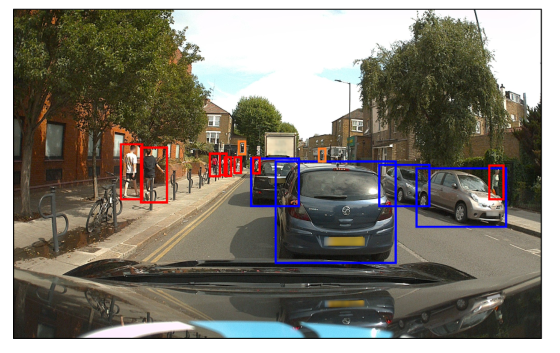
\includegraphics[width=0.4\textwidth]{ch10-4-1/figure-10-19.png}
        \caption{多个物体的边界框标注。}
    \end{figure}
\end{frame}

\begin{frame}
    \frametitle{1.2 单物体分类与定位}
    \begin{itemize}
        \item 假设图像包含\alert{一个且仅一个}来自 $C$ 个类别的物体。
        \item CNN 通常有 $C$ 个输出单元（\alert{softmax} 激活）。
        \item 额外\alert{四个输出}（\alert{线性}激活）预测边界框坐标。
        \item 边界框坐标是\alert{连续量} $\Rightarrow$ 使用\alert{平方和误差}。
    \end{itemize}
    \begin{block}{YOLO 早期思想 (Redmon et al., 2015)}
        \begin{itemize}
            \item 将图像划分为 $7 \times 7$ 网格
            \item 每个网格单元输出关联物体的类别和边界框坐标
            \item 基于来自整张图像的特征进行预测
        \end{itemize}
    \end{block}
\end{frame}

% ============================================================
% 第二部分：交并比
% ============================================================
\section{交并比}

\begin{frame}[allowframebreaks]
    \frametitle{2. 交并比 (IoU, 10.4.2)}
    \begin{itemize}
        \item 目标定位需要衡量边界框相对于\alert{真实标注}的准确度。
        \item 简单重叠面积的问题：
        \begin{itemize}
            \item 受物体大小影响
            \item 无法惩罚预测框落在真实框之外的部分
        \end{itemize}
        \item \alert{交并比 (IoU)}：交集面积与并集面积之比。
        \begin{equation}
            \text{IoU} = \frac{\text{交集面积}}{\text{并集面积}}
        \end{equation}
        \item 取值范围：\alert{0 到 1}。
        \item 通常 IoU 超过阈值 \alert{0.5} 认为预测正确。
    \end{itemize}
    \begin{figure}
        \centering
        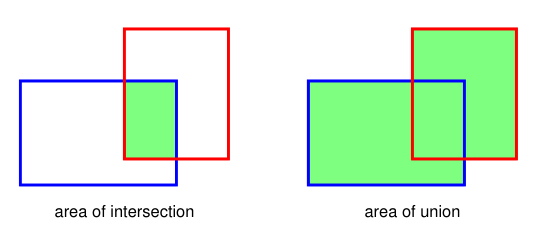
\includegraphics[width=0.35\textwidth]{ch10-4-2/figure-10-20.png}
        \caption{IoU 示意图：交集（左绿）除以并集（右绿）。}
    \end{figure}
\end{frame}

\begin{frame}
    \frametitle{2.1 IoU 的作用与局限}
    \begin{itemize}
        \item \textbf{优点}：
        \begin{itemize}
            \item 比值形式对物体大小\alert{归一化}
            \item 并集包含预测框在真实框之外的部分 $\Rightarrow$ \alert{惩罚越界预测}
        \end{itemize}
        \item \textbf{局限}：
        \begin{itemize}
            \item 一般\alert{不直接用作训练损失函数}
            \item 难以通过梯度下降优化
            \item 训练通常使用\alert{居中物体}进行
            \item IoU 主要用作\alert{评估指标}
        \end{itemize}
    \end{itemize}
\end{frame}

% ============================================================
% 第三部分：滑动窗口
% ============================================================
\section{滑动窗口}

\begin{frame}
    \frametitle{3. 滑动窗口 (10.4.3)}
    \begin{itemize}
        \item \textbf{基本思想}：
        \begin{itemize}
            \item 用紧密裁剪的物体样本 + 背景样本训练分类器
            \item 输入窗口在图像上\alert{扫描}
            \item 每个位置分类，高概率位置对应边界框
        \end{itemize}
        \item \textbf{缺点}：
        \begin{itemize}
            \item 潜在窗口位置数量\alert{巨大}，计算成本高
            \item 需多尺度窗口处理不同大小的物体
            \item 大步幅节省计算但\alert{降低定位精度}（权衡）
            \item 对百万参数的深度网络，朴素实现成本\alert{不可接受}
        \end{itemize}
    \end{itemize}
\end{frame}

\begin{frame}[allowframebreaks]
    \frametitle{3.1 卷积网络中的计算冗余}
    \begin{itemize}
        \item 卷积层本身就是\alert{滑动特征检测器}（共享权重）。
        \item 滑动窗口生成多次前向传播时，存在\alert{大量冗余计算}。
    \end{itemize}
    \begin{figure}
        \centering
        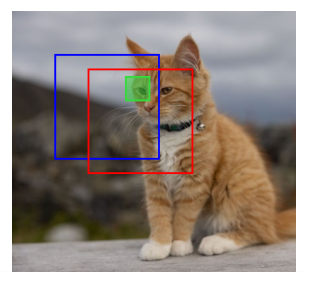
\includegraphics[width=0.3\textwidth]{ch10-4-3/figure-10-21.png}
        \caption{重叠窗口位置的计算共享（绿色感受野）。}
    \end{figure}
    \begin{itemize}
        \item \textbf{关键洞察}：滑动窗口的计算结构\alert{镜像}卷积的计算结构。
        \item 因此可在卷积网络中\alert{高效实现}滑动窗口。
    \end{itemize}
\end{frame}

\begin{frame}[allowframebreaks]
    \frametitle{3.2 简化网络示例}
    \begin{itemize}
        \item 图 10.22：卷积层 + 最大池化层 + 全连接层。
        \item 输入 $6 \times 6$，卷积层 $3 \times 3$ 步幅 1。
        \item 最大池化 $2 \times 2$ 步幅 1（不重叠感受野）。
        \item 全连接层单输出单元。
        \item \textbf{关键}：全连接层可视为\alert{滤波器大小 $2 \times 2$ 的卷积层}。
        \begin{itemize}
            \item 只有一个位置 $\Rightarrow$ 单个输出。
        \end{itemize}
    \end{itemize}
    \begin{figure}
        \centering
        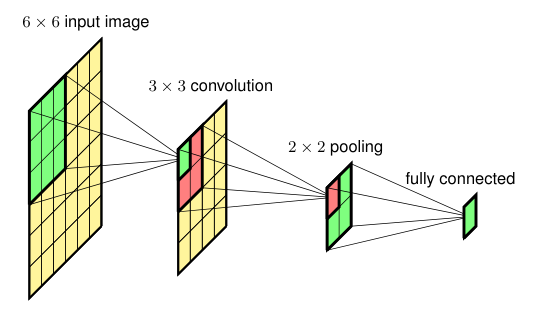
\includegraphics[width=0.4\textwidth]{ch10-4-3/figure-10-22.png}
        \caption{简单卷积网络示例。}
    \end{figure}
\end{frame}

\begin{frame}[allowframebreaks]
    \frametitle{3.3 扩大到更大图像}
    \begin{itemize}
        \item 网络在\alert{居中物体}图像上训练。
        \item 应用于更大图像（$8 \times 8$）：增大卷积和池化层大小。
        \item 卷积层：$6 \times 6$；池化层：$3 \times 3$。
        \item 得到\alert{四个输出单元}，权重共享。
        \item 处理左上角窗口的计算 = 处理原始 $6 \times 6$ 输入的计算。
        \item 其余窗口位置只需\alert{少量额外计算}（蓝色区域）。
        \item 效率显著优于朴素重复应用。
    \end{itemize}
    \begin{figure}
        \centering
        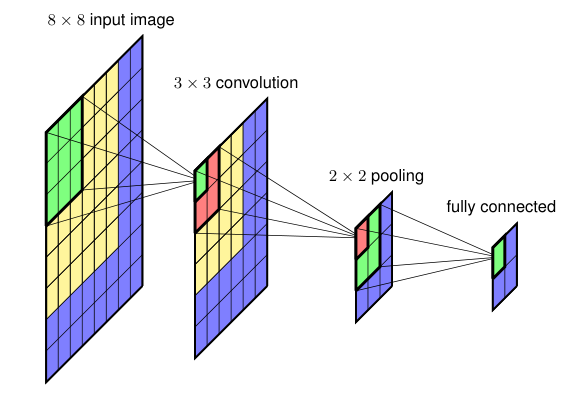
\includegraphics[width=0.4\textwidth]{ch10-4-3/figure-10-23.png}
        \caption{应用于更大图像，额外计算对应蓝色区域。}
    \end{figure}
\end{frame}

% ============================================================
% 第四部分：跨尺度检测
% ============================================================
\section{跨尺度检测}

\begin{frame}
    \frametitle{4. 跨尺度检测 (10.4.4)}
    \begin{itemize}
        \item 需在不同\alert{尺度}和\alert{宽高比}下寻找物体。
        \item 例：猫直立 vs 躺下，边界框宽高比不同。
        \item \textbf{方法}：固定输入窗口 + \alert{图像多副本缩放}。
        \begin{itemize}
            \item 制作输入图像的多个副本
            \item 每个副本有不同的水平/垂直缩放因子对
            \item 固定窗口在每个副本上扫描
            \item 用缩放因子将边界框坐标\alert{变换回原始空间}
        \end{itemize}
    \end{itemize}
    \begin{figure}
        \centering
        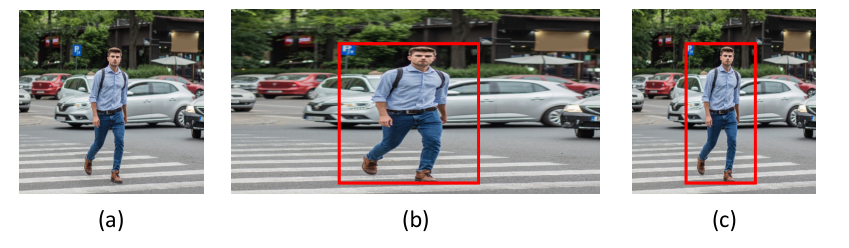
\includegraphics[width=0.5\textwidth]{ch10-4-4/figure-10-24.png}
        \caption{(a) 原图；(b) 水平缩放副本 + 检测；(c) 投影回原图。}
    \end{figure}
    \begin{itemize}
        \item 与“多尺度窗口”\alert{等价}，但实现更简单。
    \end{itemize}
\end{frame}

% ============================================================
% 第五部分：非极大值抑制
% ============================================================
\section{非极大值抑制}

\begin{frame}[allowframebreaks]
    \frametitle{5. 非极大值抑制 (10.4.5)}
    \begin{itemize}
        \item 滑动窗口扫描会产生\alert{同一物体的多次检测}（相近位置）。
        \item 通过\alert{非极大值抑制}解决，对每个类别依次执行：
    \end{itemize}
    \begin{block}{算法流程}
        \begin{enumerate}
            \item 在整个图像上运行滑动窗口，评估每个位置的类别概率
            \item 消除概率\alert{低于阈值}（如 0.7）的边界框
            \item 将\alert{概率最高}的框视为成功检测并记录
            \item 丢弃与成功检测框 \alert{IoU 超过阈值}（如 0.5）的其他框
            \item 在剩余框中重复步骤 3--4
            \item 直到所有框被丢弃或宣布为成功检测
        \end{enumerate}
    \end{block}
    \begin{figure}
        \centering
        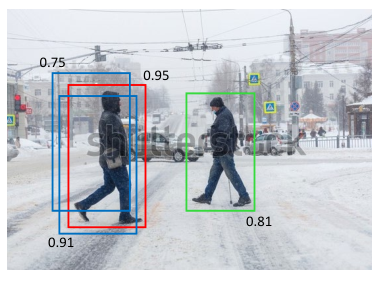
\includegraphics[width=0.4\textwidth]{ch10-4-5/figure-10-25.png}
        \caption{非极大值抑制：红框最高概率，抑制蓝框，保留绿框。}
    \end{figure}
\end{frame}

\begin{frame}
    \frametitle{5.1 两个关键阈值}
    \begin{table}
        \centering
        \renewcommand{\arraystretch}{1.3}
        \begin{tabular}{|c|c|c|}
            \hline
            \textbf{阈值} & \textbf{典型值} & \textbf{作用} \\
            \hline
            概率阈值 & 0.7 & 过滤低置信度检测 \\
            \hline
            IoU 阈值 & 0.5 & 判定重叠过多，应被抑制 \\
            \hline
        \end{tabular}
    \end{table}
    \begin{itemize}
        \item \alert{按类别独立处理}：避免不同类别相互干扰。
        \item 保留同一类别\alert{不同实例}的检测（如图中绿色框）。
        \item 位于滑动窗口和多尺度检测之后的\alert{后处理步骤}。
    \end{itemize}
\end{frame}

% ============================================================
% 第六部分：快速区域 CNN
% ============================================================
\section{快速区域 CNN}

\begin{frame}
    \frametitle{6. 快速区域 CNN (10.4.6)}
    \begin{itemize}
        \item \textbf{滑动窗口的计算浪费}：对图像所有区域应用完整深度网络。
        \item \textbf{改进思路}：先用低成本技术识别\alert{可能包含物体的区域}。
        \item \alert{快速 R-CNN} (Girshick, 2015)：
        \begin{itemize}
            \item 用分割算法等低成本技术生成区域提议
            \item 仅对这些区域应用完整网络
        \end{itemize}
        \item \alert{更快的 R-CNN} (Ren et al., 2015)：
        \begin{itemize}
            \item 使用\alert{区域提议卷积网络}识别最有希望的区域
            \item 允许区域提议网络与检测定位网络\alert{端到端训练}
        \end{itemize}
    \end{itemize}
\end{frame}

\begin{frame}
    \frametitle{6.1 滑动窗口与直接边界框预测结合}
    \begin{itemize}
        \item \textbf{滑动窗口的缺点}：精确局部化需大量密集窗口位置，计算昂贵。
        \item \textbf{更高效的方法}：结合滑动窗口与\alert{直接边界框预测}。
        \begin{itemize}
            \item 连续输出预测边界框\alert{相对于窗口位置的偏移}
            \item 对预测位置进行\alert{微调}
            \item 在保持精度的同时提高效率
        \end{itemize}
    \end{itemize}
    \begin{block}{总结：目标检测流程}
        滑动窗口 $\to$ 多尺度检测 $\to$ 非极大值抑制 $\to$ 区域提议（快速/更快的 R-CNN）
    \end{block}
\end{frame}

% ============================================================
% 第七部分：总结
% ============================================================
\section{总结}

\begin{frame}[allowframebreaks]
    \frametitle{7. 本节总结}
    \begin{itemize}
        \item \alert{边界框}：
        \begin{itemize}
            \item $\mathbf{b} = (b_x, b_y, b_W, b_H)$
            \item 单物体：$C$ 个 softmax 输出 + 4 个线性输出
            \item 平方和误差
        \end{itemize}
        \item \alert{交并比 (IoU)}：
        \begin{itemize}
            \item 交集面积 / 并集面积
            \item 范围 0 到 1，阈值 0.5
            \item 主要用作评估指标
        \end{itemize}
        \item \alert{滑动窗口}：
        \begin{itemize}
            \item 计算冗余，但可利用卷积结构高效实现
            \item 全连接层可视为卷积层
        \end{itemize}
        \item \alert{跨尺度检测}：
        \begin{itemize}
            \item 固定窗口 + 图像多副本缩放
        \end{itemize}
        \item \alert{非极大值抑制}：
        \begin{itemize}
            \item 迭代选最大概率框，抑制重叠框
            \item 概率阈值 0.7，IoU 阈值 0.5
        \end{itemize}
        \item \alert{快速/更快的 R-CNN}：
        \begin{itemize}
            \item 区域提议 + 端到端训练
            \item 滑动窗口 + 直接边界框预测
        \end{itemize}
    \end{itemize}
\end{frame}

% ============================================================
% 第八部分：参考文献
% ============================================================
\section{参考文献}

\begin{frame}
    \frametitle{8. 参考文献}
    \begin{itemize}
        \item 教材：Bishop, C. M. \& Bishop, H. (2023). Deep Learning Foundations and Concepts. Springer Nature Switzerland AG.
        \item Redmon, J. et al. (2015). You only look once: Unified, real-time object detection.
        \item Sermanet, P. et al. (2013). OverFeat: Integrated recognition, localization and detection using convolutional networks.
        \item Girshick, R. (2015). Fast R-CNN.
        \item Ren, S. et al. (2015). Faster R-CNN: Towards real-time object detection with region proposal networks.
    \end{itemize}
\end{frame}

\end{document}